\documentclass[tikz,border=2pt]{standalone}
\usepackage{amsmath,amssymb}
\usetikzlibrary{arrows.meta}
\begin{document}
% Safe pays 10 for sure; Risky pays 30 w.p. 0.4 and 0 w.p. 0.6. Expected payoffs:
% v(x) = x gives 10 vs 12 (Risky chosen); v(x) = sqrt(x) gives 3.162 vs 2.191 (Safe chosen).
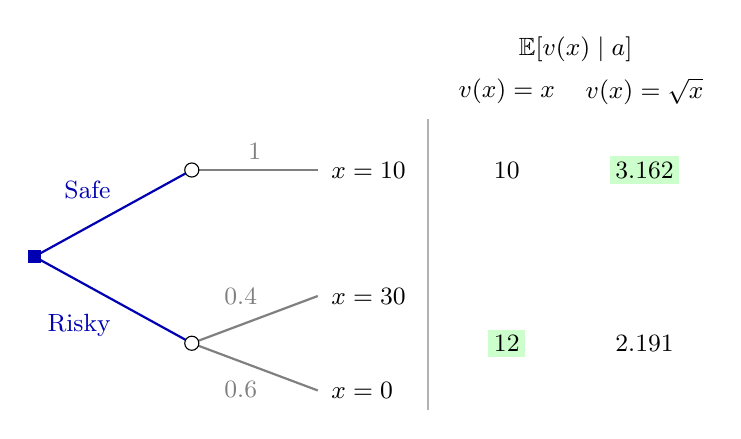
\begin{tikzpicture}[font=\small, >={Latex[length=2mm]},
    dec/.style={rectangle, fill, inner sep=2.4pt},
    chance/.style={circle, draw, fill=white, inner sep=1.8pt}]
  % tree, left to right
  \draw[blue!70!black, thick] (0,0) -- node[above left, pos=0.55] {Safe} (2.0,1.1);
  \draw[blue!70!black, thick] (0,0) -- node[below left, pos=0.55] {Risky} (2.0,-1.1);
  \draw[gray, thick] (2.0,1.1) -- node[above] {$1$} (3.6,1.1);
  \draw[gray, thick] (2.0,-1.1) -- node[above left, pos=0.6] {$0.4$} (3.6,-0.5);
  \draw[gray, thick] (2.0,-1.1) -- node[below left, pos=0.6] {$0.6$} (3.6,-1.7);
  \node[dec, blue!70!black] at (0,0) {};
  \node[chance] at (2.0,1.1) {};
  \node[chance] at (2.0,-1.1) {};
  \node[anchor=west] at (3.65,1.1) {$x=10$};
  \node[anchor=west] at (3.65,-0.5) {$x=30$};
  \node[anchor=west] at (3.65,-1.7) {$x=0$};
  % expected payoffs
  \draw[gray!60, thin] (5.0,1.75) -- (5.0,-1.95);
  \node at (6.0,2.1) {$v(x)=x$};
  \node at (7.75,2.1) {$v(x)=\sqrt{x}$};
  \node[anchor=south] at (6.875,2.35) {$\mathbb E[v(x)\mid a]$};
  \node[fill=green!20, inner sep=2pt] at (7.75,1.1) {$3.162$};
  \node at (6.0,1.1) {$10$};
  \node[fill=green!20, inner sep=2pt] at (6.0,-1.1) {$12$};
  \node at (7.75,-1.1) {$2.191$};
\end{tikzpicture}
\end{document}
